\documentclass[12pt,a4paper,titlepage]{article}
\usepackage[utf8]{inputenc}

\usepackage[left=1.5cm,right=2cm,top=2cm,bottom=2cm]{geometry}
\usepackage{amsmath}
\usepackage{amssymb}
\usepackage{amsthm}
\usepackage{hyperref}
\usepackage{graphicx}
\usepackage[space]{grffile}

\usepackage{listings}
\lstset{language=Java}


\newcommand{\class}[1]{\texttt{#1}}

\author{Jonathan Visbecq, Gaspard Férey}
\title{Projet d'INF 431 \\ - \\ Rapport}


\begin{document}
\maketitle

\tableofcontents
\newpage

\section*{Introduction}
\addcontentsline{toc}{section}{\protect\numberline{}Introduction}

Le sujet que nous avons traité proposait de s'intéresser au traitement de grande quantités de données à travers des algorithmes de comptage du nombre d'entrées différentes. Il suggérait plusieurs algorithmes que nous avons implanté, étudié et parfois modifié à la lecture des références. Parfois la liberté nous était laissée quant à l'algorithme ("Sliding Window") ou les structures de données ("Icebergs") à employer. Nous nous sommes alors appliqué à déterminer les choix qui minimisaient les coûts en temps d'exécution et en espace.\\

Nous nous sommes toujours appliqué à produire un code simple et lisible dans son implantation mais surtout cohérent dans son organisation. Ainsi les classes construites permettent d'intégrer aisément d'autres fonctions de hachage, ou de permettre le traitement d'autre types de données (texte en une autre langue, bases de données, log de serveurs web, ...) De plus, afin de travailler plus efficacement, nous avons utilisé la plateforme de travail collaboratif "GitHub". Il a donc été rapidement nécessaire de se mettre d'accord sur les bonnes pratiques à utiliser au niveau de l'organisation du code, des commentaires, de la répartition du travail,... Globalement, nous avons ainsi pu mettre à profits les nombreux enseignements tirés du cours d'INF 431 à l'origine de ce projet.\\
\\

Pour traiter le sujet, nous avons utilisé six différentes fonctions de hachage que nous avons comparé les unes par rapport aux autres. Ainsi, par exemple, nous avons observé que la fonction de hachage par défaut de Java, bien qu'elle génère peu de collisions, n'est pas parmi les plus uniforme. Les algorithmes laissent toujours le choix de la fonction de hachage à utiliser, ce qui nous a permis de contacter le réel impact négatif du choix d'une mauvaise fonction de hachage.\\

Nous avons également appliqué les différents algorithmes proposés sur des échantillons de gros textes anglais. En particulier, nous nous sommes procuré : La \textit{Bible}, \textit{Hamlet}, Un dictionnaire anglais, Le \textit{Mahabharata} complet, Les oeuvres complètes de \textit{Shakespeare}, \textit{Hamlet}, Les titres de tout les articles anglais de Wikipédia... Nous avons également généré certains gros fichiers nous-même pour bénéficier des données pseudo-aléatoires.\\

Tout nos algorithmes fonctionnent et renvoient des résultats qui nous semblent théoriquement cohérents et passent avec succès les tests que nous leur faisons subir. Ainsi :
\begin{itemize}
\item L'algorithme "HyperLogLog" renvoie des résultats cohérents, proches du nombre exact et de moins en moins éloignés plus le paramètre $b$ est grand.
La commande \class{wc} de Linux et le comptage exact via Java du résultat attendu permettent de confirmer cette précision.
\item Les similarités entre fichiers sont bien cohérentes avec leur contenu (différences de langue,...)
\item L'algorithme "Sliding Window" appliqué sur la concaténation de la Bible et des œuvres de Shakespeare a permis de détecter clairement le changement de registre lors du passage d'une œuvre à l'autre.
\item Une recherche Google avec les mots fournis par notre algorithme d'échantillonnage permet bien de retrouver immédiatement les références vers ce texte.
\end{itemize}

\newpage
\section*{Classes annexes}
\addcontentsline{toc}{section}{\protect\numberline{}Classes annexes}

\subsection*{La lecture des fichiers}

\begin{figure}
	\label{fig:fileManagerPackage}
	\centering
	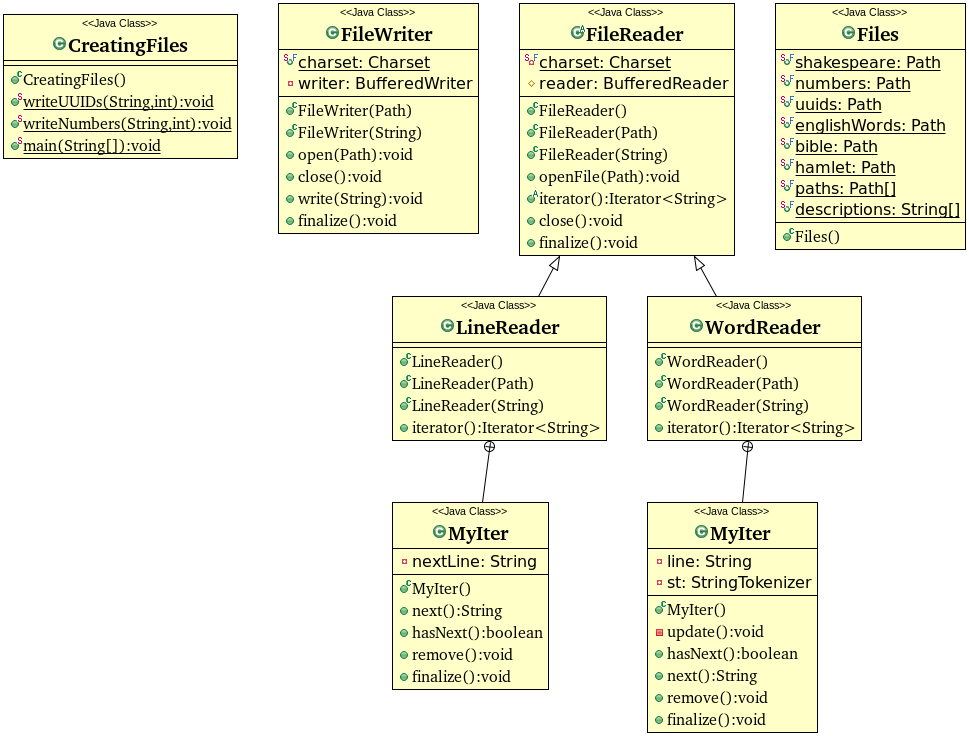
\includegraphics[scale=0.65, angle=90]{../Java Workspace/Test Hash/fileManagerPackage.png}
	\caption{Le package fileManagerPackage.}
\end{figure}

Le traitement du sujet suggère la manipulation fréquente de gros fichiers textes.\\
Les classes du package \class{FileManager} (cf diagramme \ref{fig:fileManagerPackage}) permettent de faciliter l'utilisation des fichiers. Par exemple, elles permettent de les désigner par leur chemin \class{Path} ou leur adresse \class{String} et gèrent les éventuelles exceptions lors du traitement en interne. En particulier, on y trouve :
\begin{itemize}
\item La classe abstraite \class{FileReader} qui permet d'ouvrir en lecture un fichier.\\
	Cette classe implémente l'interface \class{Iterable<String>} et permet donc de parcourir le fichier à l'aide d'une simple boucle \class{for}, rendant ainsi le code plus simple à lire.
	Elle possède deux classes filles :
	\begin{itemize}
	\item La classe \class{WordReader} qui permet de lire un fichier mot à mot.
	\item La classe \class{LineReader} qui permet de lire un fichier ligne à ligne.
	\end{itemize}
\item La classe \class{FileWriter} qui permet l'écriture dans un fichier.
\item La classe \class{Files} qui est simplement un catalogue des fichiers souvent utilisés.
\item La classe \class{CreatingFiles} qui contient des fonctions qui permettent des générer des fichiers volumineux de test. En particulier, ils permettent de génèrer :
	\begin{itemize}
	\item Un fichier des nombres de $0$ à $n$.
	\item Un fichier de $n$ identifiants UID générés par Java.
	\end{itemize}
\end{itemize}

\subsection*{L'arithmétique en Java}
La classe \class{UnsignedArithmetic} du package \class{drafts} fournit des fonctions qui permettent la correcte implantation des opérateurs addition et soustraction de deux \class{int}. En effet, Java utilise une implantation interne du type \class{int} qui préserver le bit de signe (bit de poids le plus fort) lors de certaines opérations. Les fonctions de hachage utilisées ayant recours à des entiers non signés (\textit{unsigned integers}) il nous a été nécessaire de compenser leur absence parmi les types primitifs de Java. Nous effectuons donc les opérations en se servant de \textit{long} pour contenir des entiers manipulés.

\subsection*{Communiquer}
La classe \class{Draft} du package \class{drafts} fournit, elle, des fonctions utiles à l'interface avec l'utilisateur. En particulier elle contient des méthodes d'affichage et d'utilisation de la console.




\newpage
\section{Le hachage}


Nous avons testés au début du projet plusieurs fonctions de hachage afin de déterminer le meilleur choix pour la suite. Nous avons choisit de définir chacune des fonctions de hachage comme des sous-classes de la classe abstraite \class{HashFunction} (cf diagramme \ref{fig:hashPackage}): il nous a en effet paru intuitif que que ces différentes fonctions représente un même type d'objet et ne diffèrent que par le détail de leur implémentation. Cette classe impose donc la définition des méthodes suivantes :
\begin{lstlisting}
	public int hashByteArray(byte[] array);
	public int hashString(String s);
\end{lstlisting}
dont l'implémentation dépend, bien sûr, de la fonction de hachage et qui implémentent le hachage des types de données qui nous intéressent. 

\subsection{Le hachage \class{LookUp3}}
Cette classe implante un hachage tel qu'il est décrit à adresse \href{http://www.burtleburtle.net/bob/c/lookup3.c}{http://www.burtleburtle.net/bob/c/lookup3.c}. Seuls certains détails mineurs sont à régler pour l'implémenter en Java (comme la gestion d'entiers non signés).

\subsection{Le hachage \class{MurmurHash3}}
Cette classe implante un hachage tel qu'il est décrit à adresse \href{http://en.wikipedia.org/wiki/MurmurHash}{http://en.wikipedia.org/wiki/MurmurHash}.

\subsection{Autres hachages}
Principalement pour les comparer aux deux précédents, nous avons définit d'autres fonctions de hachage :
\begin{itemize}
\item \class{DJB2} dont la description peut être trouvée à \href{http://www.cse.yorku.ca/~oz/hash.html}{http://www.cse.yorku.ca/~oz/hash.html}.
\item \class{JavaHash}, la fonction de hachage par défaut de Java.
\item \class{LoseLose}, dont la description peut être trouvée à \href{http://www.cse.yorku.ca/~oz/hash.html}{http://www.cse.yorku.ca/~oz/hash.html}.
\item \class{HomemadeHash} % au fait elle fait quoi cette fonction ?
\end{itemize}

\subsection{La classe \class{HashFunctionTests}}
Cette classe regroupe les méthodes permettant de comparer et tester les différentes fonctions de hachages.
On y trouve en particulier les méthodes suivantes :
\begin{itemize}

\item \begin{lstlisting}
private static float speedTestOnFile(Path path, HashFunction func)
\end{lstlisting}
Cette fonction parcours le fichier désigné par \class{path} et applique la fonction de hachage \class{func} sur chacun de ses mots. Elle retourne le temps que ce parcours a nécessité (en secondes). Nous désirions une fonctions suffisamment rapide pour satisfaire le cahier des charges de l'énoncé.

\item \begin{lstlisting}
public static void speedTests(Path[] paths, HashFunction func)
\end{lstlisting}
Cette fonction effectue le même test sur tout les fichiers de \class{paths} et affiche les résultats dans la sortie standard.

\item \begin{lstlisting}
private static int collisionTestOnFile(Path path, HashFunction func)
\end{lstlisting}
Cette fonction parcours le fichier désigné par \class{path} et applique la fonction de hachage \class{func} sur chacun de ses mots. Elle renvoie le nombre de collisions rencontrées entre les clefs des mots rencontrés. Nous voulions limiter au maximum les collisions, au moins entre les mots du vocabulaire anglais (puisque nos principaux fichiers de tests sont des textes en anglais).

\item \begin{lstlisting}
public static void collisionTests(Path[] paths, HashFunction func)
\end{lstlisting}
Cette fonction effectue le même test sur tout les fichiers de \class{paths} et affiche les résultats dans la sortie standard.

\item \begin{lstlisting}
private static void distributionTestOnFile(Path path, HashFunction func)
\end{lstlisting}
\label{lstlisting:distributionTestOnFile}

Cette fonction affiche l'histogramme de la distribution de la fonction de hachage \class{func} sur les mots du fichier d'adresse \class{path}. Il est ainsi possible de constater visuellement si les valeurs renvoyées par la fonction de hachage se répartissent bien uniformément. Notons que pour préserver la cohérence de l'histogramme, il faut utiliser un fichier sans doublon et contenant un échantillon le plus exhaustif possible des mots susceptibles d'être rencontrés au cours des algorithmes. De plus les mots contenus dans le fichier ne doivent pas être déjà distribués de manière aléatoire (car sinon nous obtenons toujours une distribution aléatoire, même pour une fonction de hachage de faible pertinence). Nous utilisons donc un fichier contenant un dictionnaire des mots anglais.

\item \begin{lstlisting}
private static void chiSquareTestOnFile(Path path, HashFunction func)
\end{lstlisting}
Cette fonction effectue un test du Chi-2 sur les valeurs renvoyées par la fonction de hachage sur les fichier d'adresse \class{path}. L'intervalle de confiance utilisé est de niveau 95\%. La fonction  affiche également la \textit{p-value} correspondante.

\end{itemize}

\begin{figure}
	\label{fig:hashPackage}
	\centering
	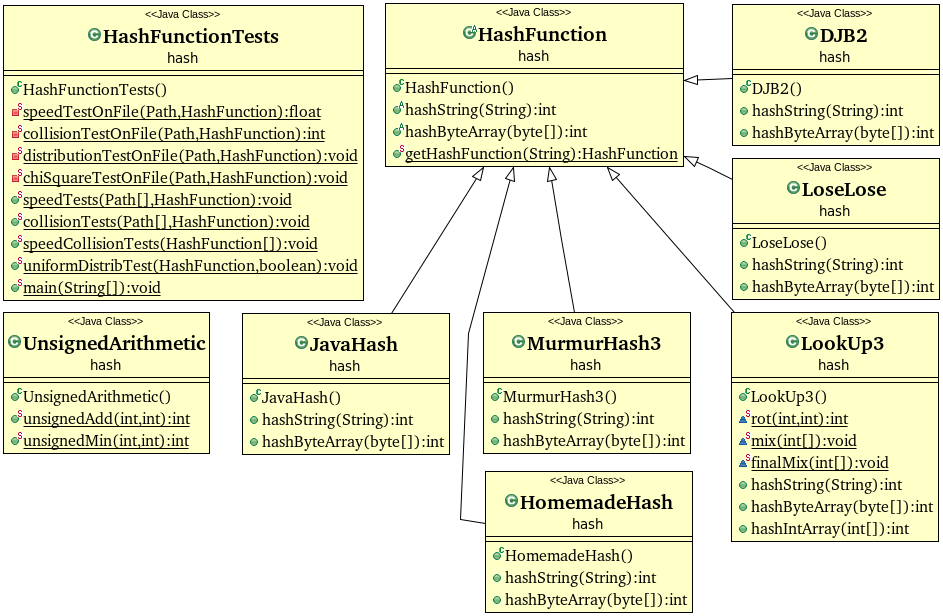
\includegraphics[scale=0.75, angle=90]{../Java Workspace/Test Hash/hashPackage.png}
	\caption{Le package \class{hash}.}
\end{figure}

\newpage
\section{L'algorithme HyperLogLog}
La classe \class{HyperLogLog} du package \class{hyperLogLog} (cf diagramme \ref{fig:hyperLogLogPackage}) contient les fonctions traitant la partie 2 du projet.\\

Les valeurs de $\alpha$ sont tabulées dans 
\begin{lstlisting}
static double[] alpha = { 0, 0.351194, 0.532435, 0.625609, ... };
\end{lstlisting}
Remarque : \class{alpha[b]} correspond à $\alpha_m$ avec $m=2^b$.\\

La fonction $\rho$ est déjà implantée en Java dans le package \class{Integer} ou elle porte le nom de \class{numberOfTrailingZeros}.
Nous fournissons également notre propre implantation :
\begin{lstlisting}
public static int rho(long x)
\end{lstlisting}

La fonction demandée en question 2 étant un cas particulier de la question 5), on décrira directement l'algorithme de la question 5), étant entendu qu'il est utilisé question 1) en prenant le paramètre $k$ égal à 1.

\subsection{Construction du tableau $M$}
Cette construction est implantée par la fonction suivante
\begin{lstlisting}
public static int[] buildFingerPrint(Path path, HashFunction func,
		int b, int k)
\end{lstlisting}
L'algorithme employé est celui décrit dans l'énoncé auquel sont apportées les modifications recommandées dans l'article de Flajolet \textit{et alii}.
En particulier les valeurs de $M$ sont initialisées à $0$ :
\begin{lstlisting}
int[] M = new int[m]; // M initialized to 0 by default
\end{lstlisting}

Pour traiter un $n$-uplet de mots, on conserve au cours de la lecture du fichier les $n$ dernier mots lus ainsi que leur taille.
Les mots sont ajoutés par
\begin{lstlisting}
strBuilder.append(s);
indexes.add(s.length());
\end{lstlisting}
et retirés par
\begin{lstlisting}
strBuilder.replace(0, indexes.poll(), "");
\end{lstlisting}



\subsection{Estimation du nombre de $k$-shingles distincts}
Le tableau $M$ construit précédemment est ensuite utilisé pour estimer le résultat selon l'algorithme spécifié dans l'énoncé. Cette estimation est stockée dans une variable \class{e}. On effectue ensuite le code suivant qui applique les modifications suggérées par l'article de Flajolet \textit{et alii}.
\begin{lstlisting}
if (e < 2.5 * m) {
    double v = 0;
    for (int i = 0; i < m; i++)
    	if (M[i] == 0) v++;
    if (v != 0)
    	e = m * Math.log(m / v);
} else if (e > n / 30)
    e = -n * Math.log(1 - e / n);
\end{lstlisting}
où $n = 2^{32}$.

\begin{figure}
	\label{fig:hyperLogLogPackage}
	\centering
	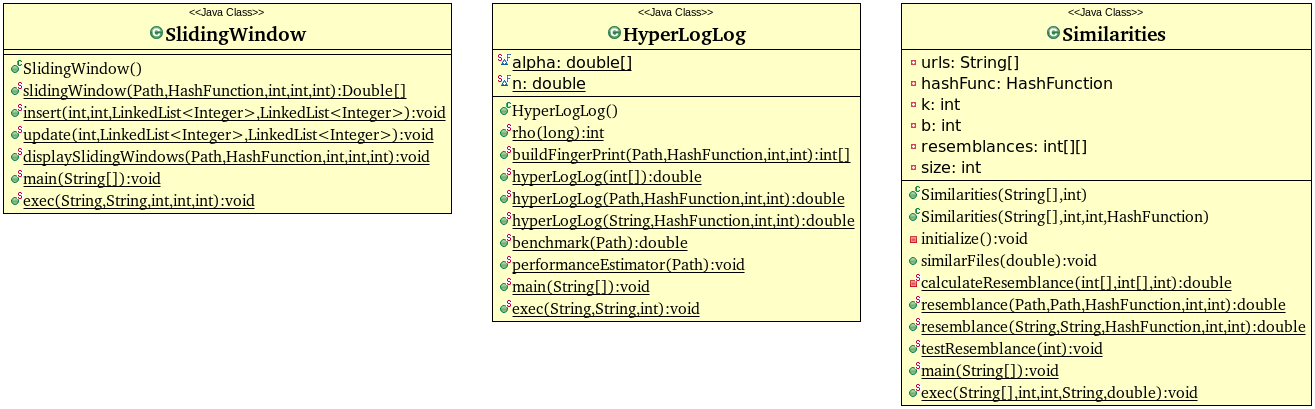
\includegraphics[scale=0.50, angle=90]{../Java Workspace/Test Hash/hyperLogLogPackage.png}
	\caption{Le package hyperLogLog.}
\end{figure}


\newpage
\section{Similarités entre ensembles de données}
Une instance de la classe \class{Similarities} (cf diagramme \ref{fig:hyperLogLogPackage}) permet de comparer deux à deux les fichiers fournit lors de sa création. L'initialisation consiste à créer les tableaux $M_i$ associés aux différents fichiers. Puis l'algorithme proposé dans l'énoncé est utilisé pour calculer la ressemblance $r(A,B)$ entre les fichiers A et B à travers la fonction
\begin{lstlisting}
private static double calculateResemblance(int[] MA, int[] MB, int b)
\end{lstlisting}
Cette fonction appliquée à toute les paires de fichiers permet déterminer lesquels présentent le plus de similarités. Nous l'avons testée, entre autres, sur des fichiers se distinguant uniquement par une centaines de mots (supprimés du fichier d'origine d'une taille de 5 Mo) avec un résultat positif.


\newpage
\section{Fenêtre glissante}
Le code permettant d'appréhender cette partie est distribué entre les classe \class{HyperLogLog} et \class{SlidingWindow} (cf diagramme \ref{fig:hyperLogLogPackage}).
On note $W$ la taille de la fenêtre.\\
L'enjeu de cet algorithme consiste à retenir à chaque instant du parcours du fichier la valeur maximale de \class{M[i]} (pour tout $i$) rencontrée lors des $W$ derniers mots. Pour cela on ne décrit pas $M$ pas un tableau d'entiers mais pas deux tableaux de listes de type \class{LinkedList<Integer>} qui sauvegardent respectivement:\\
\begin{tabular}{lcl}
\class{timestamps} &:& une valeur de $\rho$ rencontrée \\
\class{values} 	   &:& la date de la rencontre
\end{tabular}
Ceci nécessite de tenir un compteur de la date de lecture des mots.

\subsection{Insertion d'un élément}
Lors de l'insertion d'un élément $\rho$ à l'indice $i$ du tableau au temps \class{timestamp}, on consulte les deux listes $\class{values}_i$ et $\class{timestamps}_i$ :
\begin{lstlisting}
    while ( !values.isEmpty() && rho >= values.getFirst() ) {
    	values.remove();
    	timestamps.remove();
    }
    timestamps.addFirst(timestamp);
	values.addFirst(rho);
\end{lstlisting}
Ainsi on supprime tout les $\rho'$ lu précédemment qui sont inférieurs à $\rho$. En effet, ceux-ci n'ont plus aucune chance d'être le maximum de $M$ car un éléments plus grand vient d'arriver (est plus jeune dont sera supprimé après eux).
Ainsi cette insertion préserve plusieurs invariants :
\begin{itemize}
\item \class{values} et \class{timestamps} ont la même taille.
\item \class{values} est classée par ordre croissant.
\item \class{timestamps} est classé par ordre décroissant.\\
Car les \textit{timestamps} sont insérés successivement au cours de l'exécution, donc dans l'ordre croissant.
\end{itemize}

\begin{figure}[!h]
	\centering
	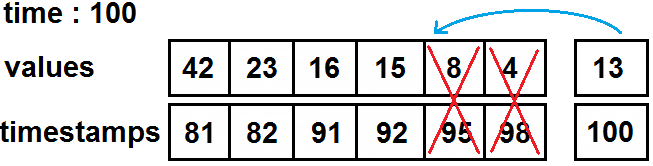
\includegraphics[scale=0.5]{pictures/picSlidingWindow2.png}
	\caption{Insertion d'un élément.}
\end{figure}

\newpage
\subsection{Nettoyage des listes}
A chaque utilisation des listes pour calculer \class{M[i]}, il faut s'assurer que le maximum a bien été suffisamment tôt. On supprime donc tout les couples (\class{timestamp}, \class{value}) qui sont plus vieux que la taille $W$ de la fenêtre. Le maximum est alors l'élément le plus vieux de la liste.

\begin{figure}[!h]
	\centering
	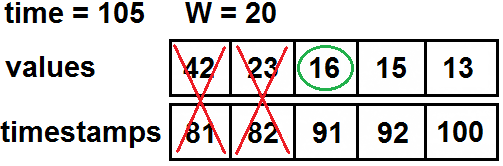
\includegraphics[scale=0.5]{pictures/picSlidingWindow1.png}
	\caption{Nettoyage des listes.}
\end{figure}

\subsection{Complexité en temps}
On effectue un passage sur tout les $N$ mots du fichier.\\
On effectue $S$ évaluations du nombre de mots distincts. A chaque évaluation il faut vérifier que les $m$ cases du tableau $M$ sont nettoyées.\\
L'ensemble des nettoyages va supprimer environ $N$ mots au total.\\

On en conclut que la complexité en temps est de $\mathcal{O}(N + mS)$. La complexité en temps reste donc linéaire à condition de ne pas être trop exigeant sur $S$.\\
Pour une représentation graphique, $S=1000$ suffit largement.

\subsection{Complexité en espace}
Le tableau $M$ ne contient plus uniquement $m$ entiers mais $2m$ listes d'entiers.\\
Cependant, ces listes ne contiennent en tout que $W+2N/S$ entiers maximum.
Les entiers de \class{timestamps} sont codés sur $\mathcal{O}(\log(N))$ bits au pire (et en moyenne).
Ceux de \class{values} sont codés sur $\mathcal{O}( \log(\log(N)) )$ bits en moyenne.
La complexité en espace est donc de $\mathcal{O}(\frac{N\log(N)}{S})$.

\subsection{Alternative}
Une alternative est d'effectuer un nettoyage supplémentaire de \class{M[i]} à chaque ajout d'une entrée à cet indice. Ainsi, la différence d'âge entre les plus vieux et plus jeunes n'excède jamais $W$ et le tableau ne peut donc pas contenir plus de $2Wm$ entiers.\\
La complexité en espace passe à $\mathcal{O}(mW\log(N))$.\\
La complexité en temps passe à  $\mathcal{O}(WN + mS)$.\\

On remarque qu'il n'est plus possible de retenir uniquement $\mathcal{O}(\log \log N)$ bits à cause de la nécessité de retenir les \class{timestamps}.
Cependant, comme il n'est pas nécessaire de retenir la date exacte, mais seulement la date relativement à la  date actuelle, on pourrait envisager d'effectuer de temps en temps une remise à jour de la date. Par exemple, comme les ages des entrées ne sont pas censées excéder $W$, on pourrait, tout les temps multiples de $W$, diminuer toutes les dates (actuelle et stockées dans $M$) de $W$. Ainsi, la complexité en temps est augmentée de $2Wm\frac{N}{W}$ mais le nombre de bit d'un \class{timestamp} devient $\mathcal{O}(\log S)$..\\
La complexité en espace passe à $\mathcal{O}(mW (\log \log N + \log W)) =^{(1)} \mathcal{O}(\log \log N)$.\\
La complexité en temps passe à $\mathcal{O}((W+m)N + mS) =^{(1)} \mathcal{O}(N)$.\\
$^{(1)}$ : Si $S$, $W$, $m$ et $N$ sont des constantes.

\newpage
\section{Mots caractéristiques}

Il s'agit, pour cette question et les suivantes, de déterminer, à partir d'un échantillonnage d'un fichier de texte, des mots vérifiant certaines propriétés statistiques. L'ensemble des classes et fonctions utiles sont regroupés au sein du package \class{sampling} (cf diagramme \ref{fig:samplingPackage}).\\

\subsection{La classe \class{Occurrence}}

Cette classe permet essentiellement de stocké un mot ainsi que son nombre d'occurrence jusqu'au point courant de lecture. Nous y redéfinissons la méthode \class{equals} de sorte que deux instances de la classe correspondent au même objet si et seulement si elle stocke le même mot. Cela permet l'utilisation correcte de la méthode \class{indexOf(Object o} de la classe \class{LinkedList<Occurrence>} dans \class{SignificantWordsSample}.


\subsection{La classe \class{SignificantWordsSample}}

Pour la recherche de mots caractéristiques, comme le sujet suggère de trouver des structures de données adaptées à l'algorithme, nous avons décidé de créer une classe abstraite \class{SignificantWordsSample} dont devront hériter chacune de nos classes représentant le sac. Cela permet de se fixer un patron que devront respecter ces classes et de séparer plus clairement leur implémentation de leur utilisation. La classe \class{SignificantWordsSample}, outre les paramètres nécessaires aux algorithmes, définit les fonctions suivantes:

\begin{itemize}
\item \begin{lstlisting}
public abstract void addWord(String string)
\end{lstlisting}
Cette fonction permet de représenter l'ajout d'un mot au sac (il s'agit d'une représentation: le mot n'est pas forcément placé dans le sac selon le fonctionnement de l'algorithme). Il s'agit d'appeler cette fonction avec pour argument chacun des mots du fichier.

\item \begin{lstlisting}
public abstract LinkedList<String> words()
\end{lstlisting}
Cette fonction permet de récupérer une liste des mots qui caractérisent le fichier dont le contenu a été transmis via \class{addWord} (au sens où ces mots sont ceux renvoyés par l'algorithme du sujet).

\item \begin{lstlisting}
public abstract double estimateMiceNumber(int nbOcc)
\end{lstlisting}
Il s'est avéré que l'échantillonnage permettant la détermination des mots caractéristiques d'un texte était identique à celui fournissant le nombre de souris (essentiellement car il s'agit principalement d'un algorithme permettant d'estimer la taille d'un fichier ou d'un flux). Seul le traitement final des données change: au lieu de renvoyer l'ensemble des mots subsistant dans le sac, on n'utilise que ceux dont le nombre d'occurrence est celui fournit en paramètre. C'est pourquoi nous retrouvons cette méthode ici.
\end{itemize}

\subsection{La classe \class{SignificantWordsSample}}

La structure de donnée utilisée lorsque l'on effectue un appel en ligne de commande (voir notice) est un tableau de 32 listes de \class{String} permettant de stocker les mots en fonction du nombre de zéros débutant l'écriture binaire de leur valeur hachée.\\
Le fonctionnement de l'algorithme est assez simple. Pour chaque mot reçu par le sac on détermine ce nombre de zéro et on ajoute le mot à la liste correspondante dans le tableau lorsque le nombre de zéros dépasse la profondeur courante $b$. Lorsque le sac est plein on supprime la liste correspondante à $b$ et on incrémente ce paramètre. De cette manière, pour une profondeur donnée b, un mot a une probabilité $2^{b}$ d'être stocké (on suppose ici que la fonction de hachage fournit des valeurs entières réparties de manière uniforme). Au fur et à mesure de l'avancement de l'algorithme b diminue et on s'attend à ce que les mots stockés soient fréquents dans le texte (car ayant un faible probabilité d'être stocké). Un appel à \class{words} (normalement lorsque le fichier a été lu entièrement) renvoie une liste de ces mots, en ne conservant que ceux dont le nombre d'occurrence est inférieur à 5 (arbitraire), ceci afin d'éviter de renvoyer des mots très fréquents non caractéristiques ('the', 'to', et c).

\subsection{Complexité en espace et en temps}

A tout instant le nombre de mots stockés est inférieur à la taille du sac: $2k$. Ces mots ont une taille variable, mais si l'espace nécessaire au stockage d'un mot (et du nombre d'occurrence) est borné par M, la complexité en espace est en $\mathcal{O}(k)$.\\

Il est difficile de déterminer la complexité en temps de l'algorithme puisqu'elle dépend de l'encombrement des listes du tableau qui, elle-même, dépend du nombre de zéros des valeurs hachées. La taille des listes est cependant bornée par la taille du sac ( $2k$ ). On lit chaque mot et on détermine à chaque fois s'il appartient à une liste d'où une complexité dans le pire cas en $\mathcal{O}(kN)$ avec N le nombre de mots lus.\\

Nous sommes bien conscients qu'une implémentation utilisant des listes force un temps linéaire à chaque fois que l'on recherche si le mot appartient à la liste (pour savoir si l'on doit augmenter ou non le nombre d'occurrences). Cependant les liste les plus longues correspondent à une profondeur faible (plus grande probabilité de commencer par peu de zéros) et donc sont inutilisées très tôt au cours de l'algorithme (car la profondeur augmente). En pratique le temps d'exécution sur le Mahâbhârata ($>$ 14 Mo) est inférieur a la seconde. Nous n'avons donc pas cherché à optimiser plus la structure.

\subsection{Autre utilisation}

Puisque les mots sont stockés à la fin de la lecture de l'algorithme dans le sac avec une probabilité $2^{b}$. Le même algorithme permet d'estimer la taille T d'un fichier ou d'un flux par
$$ T = m \times 2^{b} $$
où m est le nombre de mots du sac.

\begin{figure}
	\label{fig:samplingPackage}
	\centering
	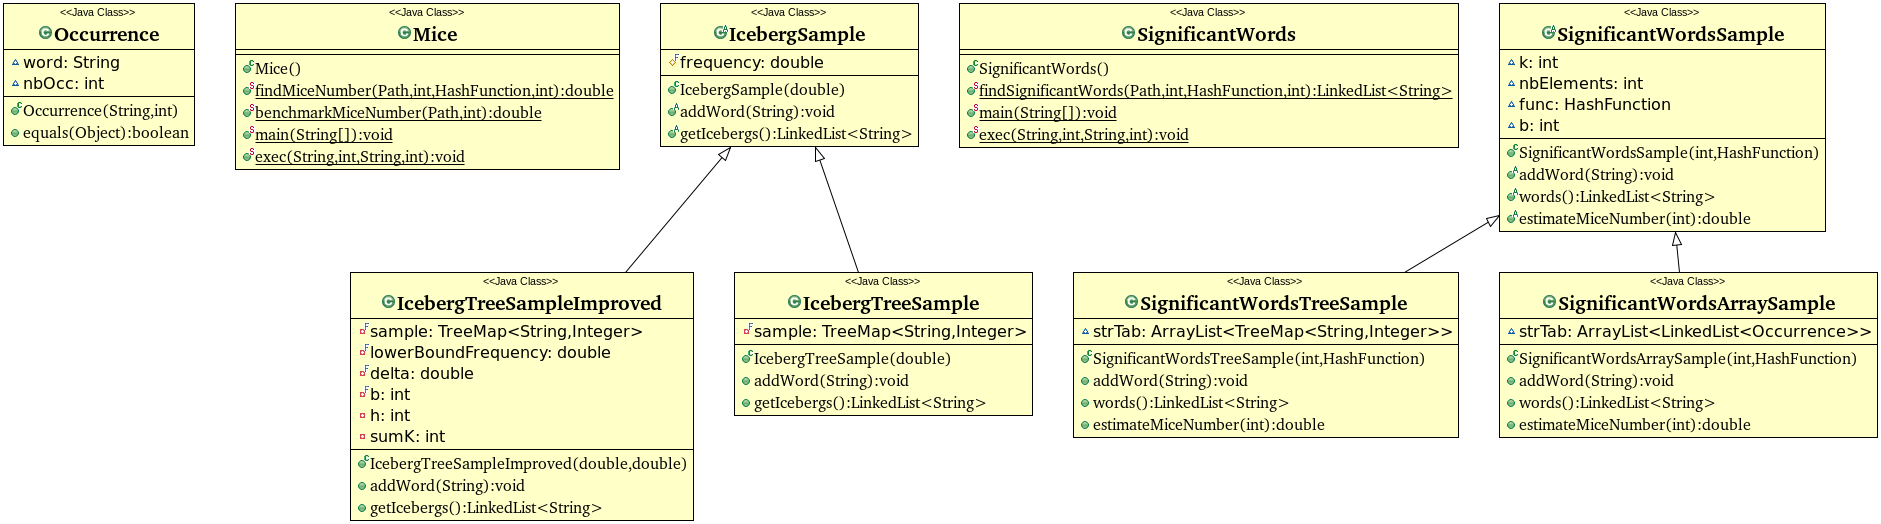
\includegraphics[scale=0.55, angle=90]{../Java Workspace/Test Hash/samplingPackage.png}
	\caption{Le package sampling.}
\end{figure}



\newpage
\section{Souris}

L'algorithme est identique au précédent. Lors de l'appel à \class{estimateMiceNumber} les mots retenus sont ceux dont le nombre d'occurrence nbOcc est celui fourni en paramètre. On suppose que la proportion de nbOcc-souris (en nombre $m_{nbOcc-souris}$) parmi les mots du sac en fin d'algorithme est identique à la proportion de nbOcc-souris dans le texte. On arrive donc à l'estimation du nombre de nbOcc-souris suivante:
$$ T_{nbOcc-souris} = m_{nbOcc-souris} \times 2^{b} $$
avec b la profondeur en fin d'algorithme.

\newpage
\section{Icebergs}

\subsection{La classe \class{IcebergSample}}

Comme pour la détermination de mots caractéristiques, puisque le sujet demande un choix approprié de structure de données et d'implémentation, nous avons crée une classe abstraite 'patron' du sac permettant l'échantillonnage (qui contient à la fois la structure de données et l'algorithme): la classe \class{IcebergSample}. Elle dispose de deux méthodes abstraites:

\begin{itemize}
\item \begin{lstlisting}
public abstract void addWord(String string)
\end{lstlisting}
Permet de faire prendre en compte un mot au sac.

\item \begin{lstlisting}
public abstract LinkedList<String> getIcebergs()
\end{lstlisting}
Permet de récupérez les icebergs.
\end{itemize}

\subsection{La classe \class{IcebergHashMapSample}}

Ce sac utilise l'algorithme dû à Karp et alii et présenté dans le sujet. Étant suffisamment simple, nous ne revenons pas dessus. Il nous fallait en revanche choisir une structure de donnée efficace. Les opérations à effectuer sur cette structure sont uniquement des ajouts, des suppressions et des tests d'appartenance. Nous ne désirons préserver aucun invariant sur les données (pas d'ordre par exemple). Pour ces raisons, une implémentation par table de hachage (type Java \class{HashMap}) nous a semblé approprié. En effet les trois opérations précédentes s'y effectuent en temps constant (temps constant amorti en vérité puisqu'il faut tenir compte des éventuels changements de capacité de la table).\\

Un exemple de résultat est fourni en annexe \ref{exemple:icebergs}. On y utilise le texte d'Hamlet.

\newpage
\section*{Conclusion}
\addcontentsline{toc}{section}{\protect\numberline{}Conclusion}


\newpage
\section*{Annexes}
\addcontentsline{toc}{section}{\protect\numberline{}Annexes}
 
\subsection*{Exemple de résultats de la recherche d'icebergs}
\label{exemple:icebergs}

\begin{verbatim}
----------------------------------------------------------------

Approximating the number of 0.03-icebergs for file:
	/home/jonathan/Documents/Projet-INF431/...
	...Java Workspace/Test Hash/files/processed/Hamlet.txt
Results :
	a
	and
	dead
	for
	hamlet
	i
	in
	is
	it
	me
	my
	of
	off
	on
	that
	the
	this
	to
	you
----------------------------------------------------------------
\end{verbatim}

\subsection*{Vrai nombre d'icebergs d'icebergs}
\label{exemple:icebergsBenchmark}

\subsection*{Exemple de résultats de la recherche d'icebergs avec l'algorithme amélioré}
\label{exemple:icebergsImproved}
 
 
 
\end{document}
